% !TeX spellcheck = en_GB
\documentclass[a4paper,11pt,oneside]{article}

\usepackage[vmargin=0.8in,outer=0.65in,inner=0.8in]{geometry}

\usepackage{newtxtext} % for roman style text and math
\usepackage{newtxmath}

\usepackage{etoolbox} % for defining and using boolean vars
\usepackage{setspace} % for changing line spacing. Using \linespread is not recommended
\usepackage{xspace} % for space after text macros
\usepackage{enumitem} % for changing settings of enumerate and itemize lists
\usepackage{caption,subcaption} % for changing caption settings
\usepackage{graphicx} % to include figures
\usepackage{float} % for modifications to figure position
\usepackage{standalone} % for stanalone tikz pictures
\usepackage{tikz}
\usetikzlibrary{arrows,calc,shapes,positioning,trees,matrix}
\usepackage{amsmath} % for math support
\usepackage{mathtools} % for math support
%\usepackage{upgreek}
\usepackage{accents}
\usepackage{empheq} % for emphasis (boxing etc) around multiple equations
\usepackage{gensymb} % for degree
\usepackage{bm} % for bold math symbols
\usepackage{cancel}
\usepackage{chemformula} % for chemicals
\usepackage{siunitx} % for units
\usepackage{booktabs} % for well spaced tables
%\usepackage{fancyhdr} % for header and footer
\usepackage{epstopdf} % for inserting .eps files as images
\usepackage[
backend=biber,
style=nature,% important, use this style only
citestyle=numeric-comp,
maxbibnames=50,
sorting=none]%important to specify this
{biblatex}
\usepackage{hyperref}
\hypersetup
{
	colorlinks=true,
	linkcolor=black,
	filecolor=black,      
	urlcolor=black,
	citecolor=black,
	pdftitle={APS-2 report},
}

\usepackage[compress,capitalize]{cleveref} % to be loaded after hyperref
% ``capitalize'' to use capital starting letter in reference
% ``compress'' to prevent sorting multiple references and use compressed referencing
\crefname{subsection}{Subsection}{Subsections} % to refer subsections, label them using \label[subsection]{name}
% Assuming that cleveref is loaded using capitalize option

\setlength{\parindent}{2em}
\setlength{\parskip}{0.5em}

\setlist[enumerate]{
	% vertical spacing
	topsep=0em,
	itemsep=0em,
	% horizontal spacing
	labelindent=0em,
	leftmargin=\parindent,
	labelsep=*,
}
\setlist[itemize]{
	% vertical spacing
	topsep=0em,
	itemsep=0em,
	% horizontal spacing
	labelindent=0em,
	leftmargin=\parindent,
	labelsep=*,
}
\captionsetup[figure]{labelfont={sf,bf},textfont={sf}}
\captionsetup[table]{labelfont={sf,bf},textfont={sf}}

%\addbibresource{references-articles.bib}
%\addbibresource{references-books.bib}
%\addbibresource{references-others.bib}

\newcommand{\newword}[1]{\textbf{#1}} % style of text for introducing a new important word or definition
\newcommand{\citear}[1]{\citeauthor{#1} \cite{#1}} % cite author and ref
\newcommand{\ndnum}[1]{\textrm{#1}} % for non-dimensional numbers
\newcommand{\vect}[1]{\ensuremath{\boldsymbol{\mathbf{#1}}}} % for 1st order tensors
\newcommand{\tens}[1]{\underline{\vect{#1}}} % for 2nd order tensors
\newcommand{\pder}[2]{\frac{\partial #1}{\partial #2}} % for partial derivative
\newcommand{\der}[2]{\frac{\sdd #1}{\sdd #2}}
\newcommand{\pprime}{{\prime\hspace{-1pt}\prime}} % double prime (only for superscripts of normal size math text. will not work for any other levels like superscript of super/subscript)
\newcommand{\ppprime}{{\prime\hspace{-1pt}\prime\hspace{-1pt}\prime}} % triple prime (only for superscripts of normal size math text. will not work for any other levels like superscript of super/subscript)
\newcommand{\norm}[1]{\left\lVert#1\right\rVert}
\newcommand{\comment}[1]{
	{\sffamily\textcolor{red}{#1}}%
} % for comments
\newcommand{\outline}[1]{
	\iftoggle{editing}{
		\noindent\rule{\linewidth}{2pt}
		\textcolor{blue!60!black}{{#1}}
		\vspace*{-1em}\noindent\rule{\linewidth}{2pt}}{
		%
	}
} % for writing outlines to sections. shows up only when 'editing' is true
\newcommand{\pens}{\textsf{pens2D}\xspace} % shortcut for pens2D
\newcommand{\plens}{\textsf{PLENS}\xspace} % shortcut for PLENS
\newcommand{\sdi}{\ensuremath{\,\text{d}}} % small 'd' for integration
\newcommand{\sdd}{\ensuremath{\text{d}}} % small 'd' for differentiation
\newcommand{\abs}[1]{\ensuremath{\left\lvert#1\right\rvert}} % absolute values
\DeclareMathOperator{\diag}{diag} % for diagonal matrices
\DeclareMathOperator{\sgn}{sgn} % sign
\newcommand{\res}{\ensuremath{\mathcal{L}}} % for residual (describing RK method)
\newcommand{\bigoh}{\ensuremath{O}} % 'order of' symbol
\newcommand{\dealii}{\textsf{deal.II}\xspace}
\newcommand{\pv}{\textsf{ParaView}\xspace}
\newcommand{\apsi}{APS-1\xspace}
\newcommand{\defeq}{\ensuremath{:=}} % defined to be equal to
\newcommand{\refelemone}{\ensuremath{\mathcal{R}}} % reference element in 1d
\newcommand{\elemmapone}{\ensuremath{\mathcal{M}}} % element mapping in 1d
\newcommand{\linalgmat}[1]{\ensuremath{\undertilde{#1}}} % for linear algebra matrix
\newcommand{\linalgvect}[1]{\ensuremath{\underline{#1}}} % linear algebra vector
\newcommand{\textdg}{\text{DG}} % text DG
\newcommand{\textfv}{\text{FV}} % text FV
\newcommand{\avg}[1]{\ensuremath{\left\{ \mskip-5mu \left\{ #1 \right\} \mskip-5mu \right\}}} % for average
\newcommand{\textch}{\text{Ch}} % abbrevation for Chandrashekhar
\newcommand{\textln}{\text{ln}} % for superscript ln in chandrashekhar flux
\newcommand{\textho}{\text{HO}} % abbrevation for high order
\newcommand{\textlo}{\text{LO}} % abbrevation for low order
\newcommand{\trouble}{\ensuremath{\mathbb{E}}} % for energy in higher modes
\newcommand{\threshold}{\ensuremath{\mathbb{T}}} % threshold for Persson's detector
\newcommand{\textmax}{\text{max}} % max in text
\newcommand{\textmin}{\text{min}} % min in text
\newcommand{\textsh}{\text{sh}} % subscript for shock impingement location in Degrez case
\newcommand{\eulerphy}[1]{\ensuremath{\mathcal{#1}}} % euler equation variables in physical space
\newcommand{\eulerref}[1]{\ensuremath{#1}} % euler equation variables in physical space
\DeclareMathOperator{\lcm}{lcm} % LCM

% Define a boolean 'editing' to have 'outline' display
\providetoggle{editing}

\addbibresource{references.bib}

\begin{document}
\onehalfspacing % line spacing set to 1.5
\raggedbottom % allow for text height to vary between pages

\tableofcontents



\section{Introduction}
\label{sec:intro}

Recently, lot of efforts are being made to bring in high order numerical methods for main-stream CFD simulations [Wang et al 2013]. One of the promising methods in this collection is the DG method. The use of DG method for nonlinear hyperbolic problems was propelled to fore-front by the work of \citear{cockburnShu1998a}. When combined with the numerical fluxes, studied in quite detail for FVM, the element-local nature of these methods makes them favourable for complex geometries and HPC \cite{cockburnShu2001}. However, they also require additional mechanisms for shock capturing and this has been the main line of work for these methods.

For a given mesh, the DG solution takes significantly higher computing time depending on the polynomial degree used. But it also gives better accuracy and resolution provided a `good' limiter is used. Instead of comparing the solutions on a given mesh, it is more useful to compare the accuracy level obtained for a given computational cost [Wang et al 2013]. In such a comparison, higher order methods perform well on cases dominated by smooth regions [refs]. However, the same comparison gives inconclusive results for flows dominated by strong discontinuities [refs].

In this work, we compare the accuracy and computational cost for 4 different polynomial interpolation values. In doing this, we keep the degrees of freedom constant which results in a constant memory load on the CPU. We aim to study and conclude what type of cases have advantageous high order solutions. We also aim to answer to what extent will increasing polynomial order significantly effect the accuracy of the solution, and when does the computational cost offset any benefit in this regard.



\section{Governing equations}
\label{sec:gov-eq}

This work simulates the 3d Euler equations given by
\begin{equation*}
	\pder{\vect{\eulerphy{U}}}{t} + \sum_{i=1}^{3} \pder{\vect{\eulerphy{F}}_i}{x_i} = \vect{0},
	\label{eq:3d_euler}
\end{equation*}
where $\vect{\eulerphy{U}} \defeq \left[ \rho\ \rho u_1\ \rho u_2\ \rho u_3\ \rho E \right]^T$ is the state vector, and the flux vectors are given by
\begin{equation*}
	\vect{\eulerphy{F}}_i(\vect{\eulerphy{U}}) \defeq
	\begin{bmatrix}
		\rho u_i\\
		\rho u_1 u_i\\
		\rho u_2 u_i\\
		\rho u_3 u_i\\
		\rho E u_i
	\end{bmatrix}
	+ p
	\begin{bmatrix}
		0\\
		\delta_{1i}\\
		\delta_{2i}\\
		\delta_{3i}\\
		u_i
	\end{bmatrix}
	\label{eq:3d_euler_flux_tensor}
\end{equation*}
Here, $\rho$ and $p$ represent density and pressure respectively, $u_i$ are the velocity components, and $\delta_{ij}$ is the Kronecker delta. The total energy $E \defeq e + \frac{q^2}{2}$ where $q$ is the specific kinetic energy and $e \defeq (\gamma-1)p/\rho$ for a calorically perfect gas with specific heat ratio $\gamma$.



\section{Numerical method}
\label{sec:num_method}

The split form DGSEM algorithm \cite{gassnerWintersKopriva2016} along with the subcell limiter of \citear{hennemannRamirezHindenlang2021} is used. The algorithm is described here in brief for the 1d system of equations
\begin{equation}
	\pder{\vect{\eulerphy{U}}}{t} + \pder{\vect{\eulerphy{F}}_1}{x_1} = \vect{0} \quad (t \geq 0,\ x_1 \in \Omega).
	\label{eq:1d_euler}
\end{equation}
For simplicity, the subscript `1' is dropped in this section. The domain $\Omega$ is partitioned into non-overlapping 1d elements, $\{\Omega_e\}_{e=0}^{N_e-1}$. Consider the restriction of \cref{eq:1d_euler} to a representative element $\Omega_e \defeq [a,b]$ which is being mapped to the reference element $\refelemone \defeq [0,1]$ using the linear mapping $\xi \xmapsto{\elemmapone} x$:
\begin{gather*}
	\elemmapone^{-1}(x) = \xi = \frac{x-a}{b-a} \quad (x \in \Omega_e \defeq [a,b]),
	\label{eq:1d_element_mapping}\\
	J \pder{\vect{\eulerref{U}}}{t} + \pder{\vect{\eulerref{F}}}{\xi} = \vect{0} \quad (t \geq 0,\ \xi \in \refelemone \defeq [0,1]),
	\label{eq:1d_euler_refelem}
\end{gather*}
where $\vect{\eulerref{U}}(\xi,t) \defeq \vect{\eulerphy{U}}(x,t)$, $\vect{\eulerref{F}}(\vect{\eulerref{U}}) \defeq \vect{\eulerphy{F}}(\vect{\eulerref{U}})$ are the conservative state and flux in reference space, and $J \defeq \sdd \elemmapone/\sdd \xi = (b-a)$ is the Jacobian of the mapping. $\vect{\eulerref{U}}$ and $\vect{\eulerref{F}}$ are approximated to lie in a linear polynomial space of $N$-th degree polynomials
\begin{equation*}
	\vect{\eulerref{U}}(\xi,t) \approx \sum_{i=0}^{N} \vect{\eulerref{U}}_i(t) \ell_i(\xi), \quad \eulerref{\vect{F}}(\xi,t) \approx \sum_{i=0}^{N} \eulerref{\vect{F}}(\vect{\eulerref{U}}_i(t)) \ell_i(\xi),
	\label{eq:1d_euler_state_flux_interpolation}
\end{equation*}
where $\{\ell_i(\xi)\}_{i=0}^{N}$ are the basis Lagrange functions constructed using the $(N+1)$ Gauss-Lobatto (GL) points as nodes, and $\{\vect{\eulerref{U}}_i\}_{i=0}^{N}$ are the nodal values. The error in this approximation is minimised using the Galerkin approach in a strong sense for the test functions $\{\ell_j\}_{j=0}^{N}$:
\begin{equation}
	\int_{0}^{1} \ell_j J \pder{\vect{\eulerref{U}}}{t} \sdi \xi + \int_{0}^{1} \ell_j \pder{\vect{\eulerref{F}}}{\xi} \sdi \xi + \left[\ell_j (\vect{\eulerref{F}}^*-\vect{\eulerref{F}}) \right]_{\xi=0}^{\xi=1} = \vect{0}\quad (j=0,1,\ldots,N),
	\label{eq:1d_euler_strong_form}
\end{equation}
where $\vect{\eulerref{F}}^*$ is the numerical flux function introduced at the element boundaries to ensure conservation. \cref{eq:1d_euler_strong_form} can be simplified by introducing the \newword{mass} and \newword{stiffness} matrices, $\linalgmat{M}$ and $\linalgmat{S}$
\begin{equation}
	\sum_{j=0}^{N} M_{ij} J \dot{\vect{\eulerref{U}}}_j + S_{ij} \vect{\eulerref{F}}_j + B_{ij} \left( \vect{\eulerref{F}}^*_j - \vect{\eulerref{F}}_j \right) = 0 \quad (i=0,1,\ldots,N),
	\label{eq:1d_euler_tensor_form1}
\end{equation}
where $\vect{\eulerref{F}}_j=\eulerref{\vect{F}}(\vect{\eulerref{U}}_j)$, $\vect{\eulerref{F}}^*_j$ is the inter-element numerical flux (non-zero only for $j=0,N$),
\begin{gather*}
	M_{ij} \defeq \int_{0}^{1} \ell_i \ell_j \sdi \xi \quad (i,j=0,1,\ldots,N),\\
	S_{ij} \defeq \int_{0}^{1} \ell_i \der{\ell_j}{\xi} \sdi \xi \quad (i,j=0,1,\ldots,N),
\end{gather*}
and $\linalgmat{B} \defeq \diag (-1,\ 0,\ \ldots,\ 0,\ 1)$ is the surface evaluation matrix of size $(N+1)$ as well.

The DGSEM uses co-located quadrature to evaluate mass and stiffness matrices which simplifies the matrix element expressions, and also the strong form discretization given in \cref{eq:1d_euler_tensor_form1} as follows
\begin{gather}
	\linalgmat{M} = \diag(w_0,\ w_1,\ \ldots,\ w_N),
	\label{eq:dgsem_mass_matrix} \nonumber\\
	\linalgmat{S} = \linalgmat{M} \linalgmat{D}, \quad D_{ij} = \der{\ell_j}{\xi}(\xi_i) \quad (i=0,1,\ldots,N),
	\label{eq:dgsem_polynomial_derivative_matrix} \nonumber\\
	J \dot{\vect{\eulerref{U}}}_i + \sum_{j=0}^{N} \left[ D_{ij} \vect{\eulerref{F}}_j \right] - \frac{\delta_{0i}}{w_0} \left( \vect{\eulerref{F}}^*_0 - \vect{\eulerref{F}}_0 \right) + \frac{\delta_{Ni}}{w_N} \left( \vect{\eulerref{F}}^*_N - \vect{\eulerref{F}}_N \right) = 0 \quad (i=0,1,\ldots,N),
	\label{eq:1d_euler_tensor_form2}
\end{gather}
where $\{w_i\}_{i=0}^{N}$ are the weights of the GL quadrature and $\linalgmat{D}$ is the \newword{polynomial derivative} matrix. The co-located quadrature also gives summation-by-parts property to $\linalgmat{S}$ which allows writing the volumetric term of \cref{eq:1d_euler_tensor_form2} as a FV flux difference \cite{fisherCarpenterNordstrom2013}:
\begin{equation}
	\sum_{j=0}^{N} D_{ij} \vect{\eulerref{F}}_j = \frac{\hat{\vect{\eulerref{F}}}_{i+1} - \hat{\vect{\eulerref{F}}}_i}{w_i} \quad (i=0,1,\ldots,N),
	\label{eq:telescopic_form}
\end{equation}
where $\{\hat{\vect{\eulerref{F}}}_i\}_{i=0}^{N+1}$ are the corresponding consistent volumetric fluxes defined on the \newword{flux points} $\{\hat{\xi}_i\}_{i=0}^{N+1}$. This gives an effective subcell decomposition for every element which is visually shown in \cref{fig:dgsem_subcell_fc_equivalence}. These flux points are related to the quadrature (or interpolation) points through the weights as follows.
\begin{equation*}
	\hat{\xi}_0 = \xi_0; \quad \hat{\xi}_{N+1} = \xi_N;\quad
	\hat{\xi}_{i+1} - \hat{\xi}_i = w_i\ \  (i=0,1,\ldots,N)
	\label{eq:flux_points}
\end{equation*}
\begin{figure}[htbp]
	\centering
	\includestandalone{figures/dgsem_subcell_fv_equivalence}
	\caption{Equivalent subcell FV decomposition for a DGSEM element with $N=3$. Figure shows the GL interpolation (or quadrature) nodes (circles) and the flux points (crosses). In this case, 4 subcells of sizes $w_0,\ w_1,\ w_2$ and $w_3$ between 5 flux points are obtained.}
	\label{fig:dgsem_subcell_fc_equivalence}
\end{figure}
While the relation between volumetric fluxes ($\{\hat{\vect{\eulerref{F}}}_i\}_{i=0}^{N+1}$) and nodal fluxes ($\{\vect{\eulerref{F}}_j\}_{j=0}^{N}$) is given in \cite{fisherCarpenterNordstrom2013}, \citear{gassnerWintersKopriva2016} (extending the work of \citear{fisherCarpenter2013}) suggested the \newword{split form} DGSEM, in which the volumetric fluxes are constructed independent of nodal fluxes using
\begin{equation}
	\begin{gathered}
		\hat{\vect{\eulerref{F}}}_0 \approx \vect{\eulerref{F}}_0, \quad \hat{\vect{\eulerref{F}}}_{N+1} \approx \vect{\eulerref{F}}_N,\\
		\hat{\vect{\eulerref{F}}}_i \approx \sum_{j=i}^{N} \sum_{k=0}^{i-1} 2 w_k D_{kj} \vect{\eulerref{F}}^\#(\vect{\eulerref{U}}_k, \vect{\eulerref{U}}_j)\quad (i=1,2,\ldots,N),
	\end{gathered}
	\label{eq:split_form_subcell_flux}
\end{equation}
where $\vect{\eulerref{F}}^\#$ is a \newword{volumetric two-point flux function}. Substituting \cref{eq:split_form_subcell_flux,eq:telescopic_form} in \cref{eq:1d_euler_tensor_form2}, the split-form DGSEM discretization can be written as follows.
\begin{equation}
	J \dot{\vect{\eulerref{U}}}_i + 2\sum_{j=0}^{N} D_{ij} \vect{\eulerref{F}}^\#(\vect{\eulerref{U}}_i, \vect{\eulerref{U}}_j) - \frac{\delta_{0i}}{w_0} \left( \vect{\eulerref{F}}^*_0 - \vect{\eulerref{F}}_0 \right) + \frac{\delta_{Ni}}{w_N} \left( \vect{\eulerref{F}}^*_N - \vect{\eulerref{F}}_N \right) = 0 \quad (i=0,1,\ldots,N)
	\label{eq:1d_euler_tensor_form3}
\end{equation}

\citear{hennemannRamirezHindenlang2021} proposed a limiting technique where the split-form high order DGSEM scheme is blended with a low order scheme. Since the introduction of flux points and volumetric fluxes (\cref{eq:telescopic_form,fig:dgsem_subcell_fc_equivalence}) provides a natural subcell decomposition of the finite element, the low order scheme was constructed by defining the volumetric fluxes using standard numerical flux as follows.
\begin{equation}
	\begin{gathered}
		\hat{\vect{\eulerref{F}}}^\textlo_0 \approx \vect{\eulerref{F}}_0, \quad \hat{\vect{\eulerref{F}}}^\textlo_{N+1} \approx \vect{\eulerref{F}}_N,\\
		\hat{\vect{\eulerref{F}}}^\textlo_i \approx \vect{\eulerref{F}}^*(\vect{\eulerref{U}}_{i-1}, \vect{\eulerref{U}}_i)\quad (i=1,2,\ldots,N),
	\end{gathered}
	\label{eq:low_order_subcell_flux}
\end{equation}
Using \cref{eq:low_order_subcell_flux,eq:telescopic_form} in \cref{eq:1d_euler_tensor_form2} gives a first order subcell discretization, which is blended with the high order discretization (\cref{eq:1d_euler_tensor_form3}) using a factor $\alpha$.
\begin{equation}
	\begin{aligned}
		J \dot{\vect{\eulerref{U}}}_i + (1-\alpha) \sum_{j=0}^{N} 2 D_{ij} \vect{\eulerref{F}}^\#(\vect{\eulerref{U}}_i, \vect{\eulerref{U}}_j) + \alpha \frac{\hat{\vect{\eulerref{F}}}^\textlo_{i+1} - \hat{\vect{\eulerref{F}}}^\textlo_i}{w_i} &-\\
		\frac{\delta_{0i}}{w_0} \left( \vect{\eulerref{F}}^*_0 - \vect{\eulerref{F}}_0 \right) + \frac{\delta_{Ni}}{w_N} \left( \vect{\eulerref{F}}^*_N - \vect{\eulerref{F}}_N \right) &= 0 \quad (i=0,1,\ldots,N)
	\end{aligned}
	\label{eq:1d_euler_tensor_form4}
\end{equation}
A modification of the energy indicator of \citear{perssonPeraire2006} is used to calculate $\alpha$. Following \cite{hennemannRamirezHindenlang2021}, in this work, the variable the product of pressure and density ($p\rho$) is used calculate $\alpha$ and its value is capped at $\alpha_\textmax=0.5$ unless mentioned otherwise.

The boundary conditions for all problems are applied in a `weak-Riemann' sense, following the approach of \citear{mengaldoDeGraziaPeiro2014}.

\subsection{Choice of volume and surface fluxes}
\label{subsec:vol_surf_flux}
In this work, the Chandrashekhar volumetric flux \cite{gassnerWintersKopriva2016,chandrashekar2013} is used,
\begin{equation*}
	\vect{\eulerref{F}}^\#_\textch(\vect{\eulerref{U}}_a, \vect{\eulerref{U}}_b) =
	\begin{bmatrix}
		\rho^\textln \avg{u_1} \\
		\rho^\textln \avg{u_1}^2 + \dfrac{\avg{\rho}}{2\avg{\beta}} \\
		\rho^\textln \avg{u_1} \avg{u_2} \\
		\rho^\textln \avg{u_1} \avg{u_3} \\
		\rho^\textln \avg{u_1} \left( \dfrac{1}{2\beta^\textln (\gamma-1)} + \dfrac{\avg{\rho}}{2\rho^\textln \avg{\beta}} + \sum\limits_{i=1}^{3} \left[ \avg{u_i}^2 - \dfrac{1}{2} \avg{u_i^2} \right] \right)
	\end{bmatrix},
	\label{eq:1d_chandrashekhar_volume_flux}
\end{equation*}
where $\avg{x} \defeq (x_a + x_b)/2$, $x^\textln \defeq (x_a - x_b)/(\ln (x_a/x_b))$ and $\beta = \rho/2p$. A numerically stable procedure to calculate the logarithmic averages is given in the appendix of \cite{ismailRoe2009}. The numerical surface flux $\vect{\eulerref{F}}^*$, is obtained by adding a stabilisation (dissipation) term to the volume flux. In this work, the hybrid matrix based stabilisation \cite{chandrashekar2013} is used to obtain the surface flux,
\begin{gather}
	\vect{\eulerref{F}}^*(\vect{\eulerref{U}}_a, \vect{\eulerref{U}}_b) = \vect{\eulerref{F}}^\#_\textch(\vect{\eulerref{U}}_a, \vect{\eulerref{U}}_b) - \frac{1}{2} \vect{K} \abs{\vect{\Lambda}} \vect{K}^{-1} \left( \vect{\eulerref{U}}_b - \vect{\eulerref{U}}_a \right),\\
	\abs{\vect{\Lambda}} = \alpha \abs{\vect{\Lambda}}^\text{Rusanov} + (1-\alpha) \abs{\vect{\Lambda}}^\text{Roe},\\
	\abs{\vect{\Lambda}}^\text{Rusanov} = (\abs{\tilde{u}_1} + \tilde{a}) \vect{I},\\
	\abs{\vect{\Lambda}}^\text{Roe} = \diag \left( \abs{\tilde{u}_1 - \tilde{a}}, \abs{\tilde{u}_1}, \abs{\tilde{u}_1}, \abs{\tilde{u}_1}, \abs{\tilde{u}_1 + \tilde{a}} \right)
	\label{eq:1d_chandrashekhar_surface_flux}
\end{gather}
where superscript $\sim$ is used to denote Roe-averaged quantities, $\vect{K}$ is the right eigenvector matrix of Roe-averaged state and $\vect{I}$ is the identity matrix of size 5.



\section{One-dimensional test results}
\label{sec:1d_tests}

Five Riemann 1d problems taken from \citear{toro2009} are considered for comparing performance of polynomial degrees $N=1,\ 2,\ 3$ and $5$. The initial conditions for these tests are given \cref{tab:ic_riemann1d}. The problems were setup on a 3d domain $[0,1] \times [0,0.5]^2$ with $\lcm \{N+1 \mid N=1,2,3,5\}=12$ DoFs in $y$ and $z$ directions. Three sets of simulations on three grid resolutions for $x$ direction were performed with the number of cells given in \cref{tab:nx_riemann1d}. Explicit 5-stage RK4 time integrator \cite{kennedyCarpenterLewis2000} is used with a CFL number of 0.5.

\begin{table}[htbp]
	\centering
	\caption{Initial conditions for Riemann 1d problems. All values in SI units. The diaphragm location ($x_0$) is where the initial discontinuity is set.}
	\label{tab:ic_riemann1d}
	\begin{tabular}{c c c c c c c c c}
		\toprule
		Test \# & $\rho_L$ & $\rho_R$ & $p_L$ & $p_R$ & $u_L$ & $u_R$ & End time & $x_0$ \\ \midrule
		1 & 1.0 & 0.125 & 1.0 & 0.1 & 0.75 & 0.0 & 0.2 & 0.3 \\
		2 & 1.0 & 1.0 & 0.4 & 0.4 & -2.0 & 2.0 & 0.15 & 0.5 \\
		3 & 1.0 & 1.0 & 1000.0 & 0.01 & 0.0 & 0.0 & 0.012 & 0.5 \\
		4 & 5.99924 & 5.99242 & 460.894 & 46.095 & 19.5975 & -6.19633 & 0.035 & 0.3 \\
		5 & 1.0 & 1.0 & 1000.0 & 0.01 & -19.59745 & -19.59745 & 0.012 & 0.8 \\
		\bottomrule
	\end{tabular}
\end{table}

\begin{table}[htbp]
\centering
\caption{Number of cells in $x$ direction for Riemann 1d problems.}
\label{tab:nx_riemann1d}
\begin{tabular}{lllll}
	\toprule
	Nominal DoFs & $N=1$ & $N=2$ & $N=3$ & $N=5$\\
	\midrule
	200 & 100 & 66 & 50 & 34 \\
	400 & 200 & 134 & 100 & 66 \\
	800 & 400 & 266 & 200 & 134 \\
	\bottomrule
\end{tabular}
\end{table}

All simulations were performed on a \comment{machine specs}. The simulation results and the exact solution are sampled at 6400 equidistant points to calculate the $L^2$ error as
\begin{equation*}
\frac{\norm{\phi_\text{numerical} - \phi_\text{exact}}_{L^2}}{\norm{\phi_\text{exact}}_{L^2}}
\end{equation*}
where $\norm{\bullet}_{L^2}$ represents the $L^2$ norm and $\phi=\rho$ for all cases except Test 2 for which $\phi=T$.

\subsection{Test 1}
\label{subsec:test1-1}

This is a relatively mild test with weak right-moving contact and shock waves, and an expansion wave with left-moving head and right-moving tail, thus producing a sonic point in the expansion wave. \cref{fig:test1-1_dof800_chandrashekhar} shows a visual comparison of the results obtained using $N=1,\ 2,\ 3$ and $5$ at the highest resolution (800 DoFs). All simulations capture the sonic point and the shock well, while the resolution of contact wave gets better with increasing $N$. Behaviour of the error in simulations with increasing DoFs for different values of $N$ is shown in \cref{fig:test1-1_error_plots_chandrashekhar}. It is immediately clear from \cref{subfig:test1-1_error_vs_dof_chandrashekhar} that even high order simulations fail to achieve higher order of convergence in this discontinuous flow. \cref{subfig:test1-1_error_vs_dof_chandrashekhar,subfig:test1-1_error_vs_cputime_chandrashekhar} together show that there is no major improvement in solution when $N=5$ is used over $N=3$, although it costs more CPU time. The error levels for $N=3,5$ are much lower compared to $N=1$ case. \cref{subfig:test1-1_error_vs_cputime_chandrashekhar} also shows that with very small increase in cost, $N=3$ offers more accurate solution over $N=2$. It may be concluded that $N=3$ would be the optimal choice for this case.

\begin{figure}[htbp]
	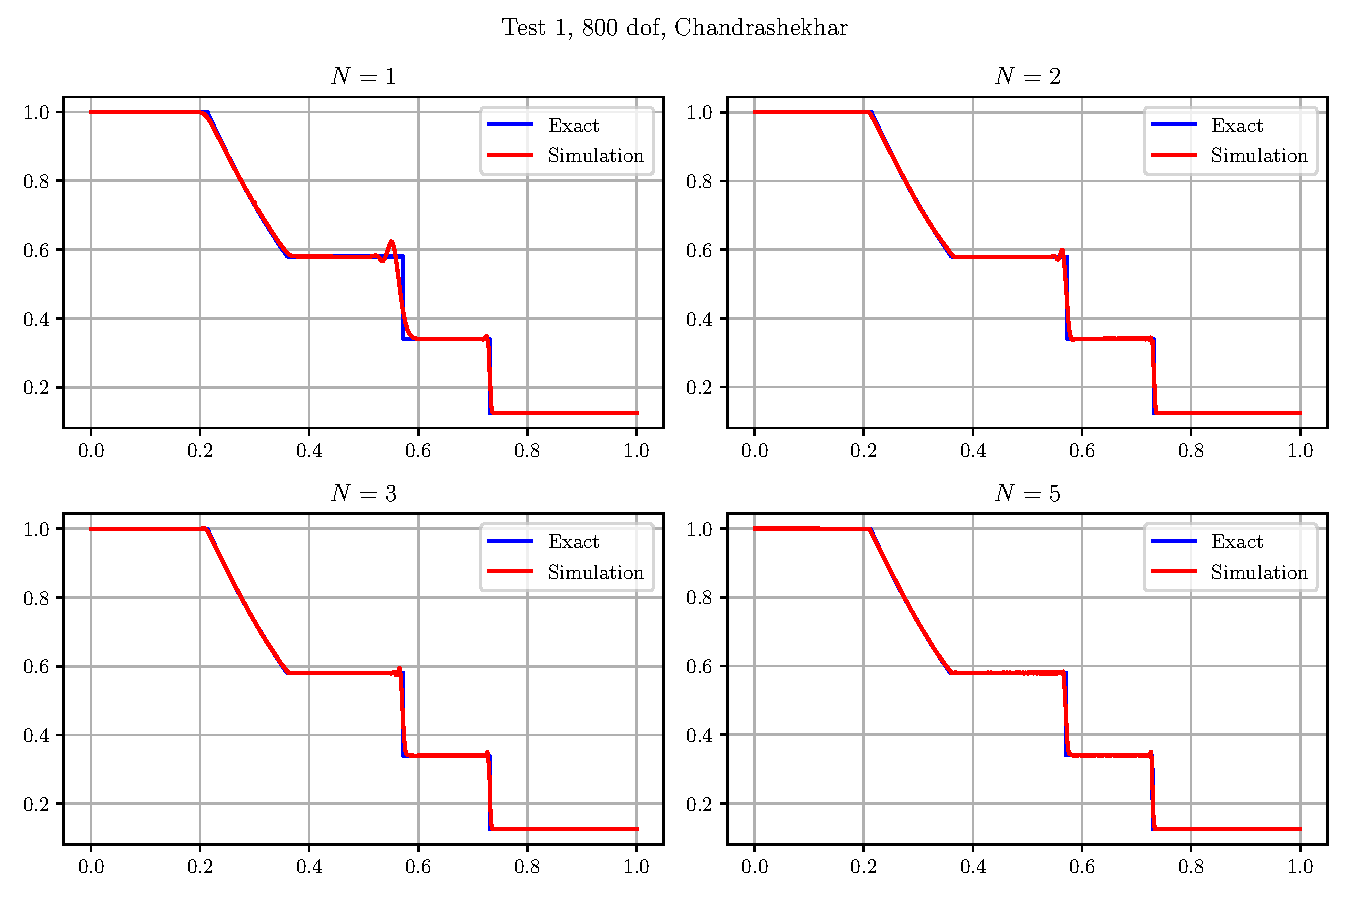
\includegraphics[width=\linewidth]{figures/riemann_1d/test1-1/dof800_12_12_chandrashekhar.pdf}
	\caption{Comparison of results for 800 DoFs, Test 1.}
	\label{fig:test1-1_dof800_chandrashekhar}
\end{figure}

\begin{figure}[htbp]
	\centering
	\begin{subfigure}{0.5\linewidth}
		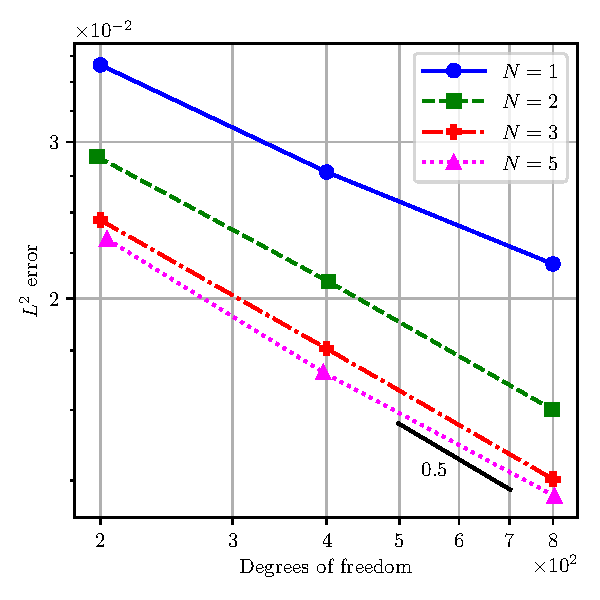
\includegraphics[width=\linewidth]{figures/riemann_1d/test1-1/error_vs_dof_chandrashekhar.pdf}
		\caption{Error vs DoFs.}
		\label{subfig:test1-1_error_vs_dof_chandrashekhar}
	\end{subfigure}%
	\begin{subfigure}{0.5\linewidth}
		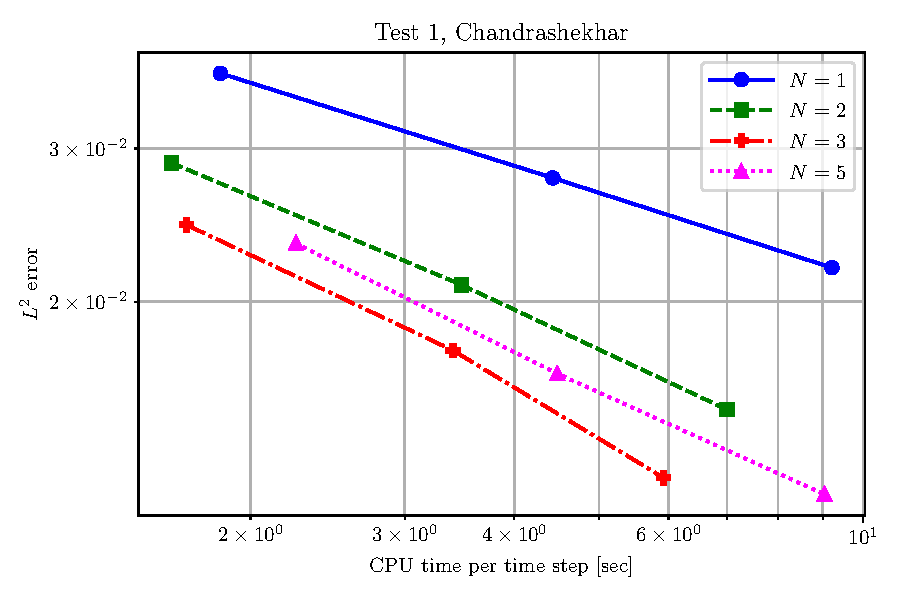
\includegraphics[width=\linewidth]{figures/riemann_1d/test1-1/error_vs_cputime_chandrashekhar.pdf}
		\caption{Error vs CPU time.}
		\label{subfig:test1-1_error_vs_cputime_chandrashekhar}
	\end{subfigure}
	\caption{Statistics for Test 1.}
	\label{fig:test1-1_error_plots_chandrashekhar}
\end{figure}

\printbibliography
\end{document}